\resizebox{\figurewidth}{\figureheight}{
 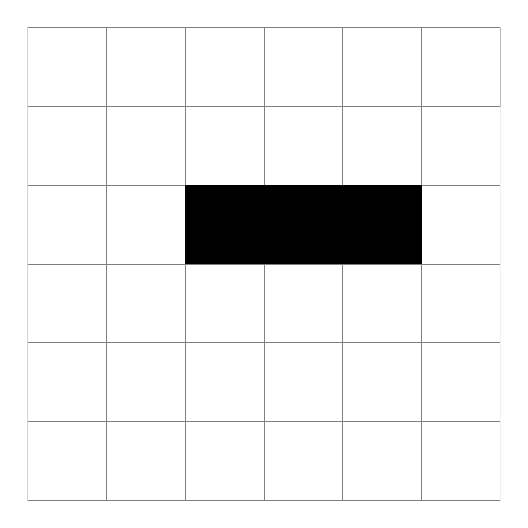
\begin{tikzpicture}
    \clip (-1,-1) rectangle (5cm,5cm); % Clips the picture...

    \draw[style=help lines] (-14,-14) grid[step=\cacellsize] (14,14);
    \draw [fill=black] (1\cacellsize,2\cacellsize) rectangle (2\cacellsize,3\cacellsize);
    \draw [fill=black] (2\cacellsize,2\cacellsize) rectangle (3\cacellsize,3\cacellsize);
	\draw [fill=black] (3\cacellsize,2\cacellsize) rectangle (4\cacellsize,3\cacellsize);
	\draw [fill=black] (5\cacellsize,4\cacellsize) rectangle (6\cacellsize,5\cacellsize);
  \end{tikzpicture}
}
